\documentclass[12pt,a4paper]{article}
\usepackage[utf8]{inputenc}
\usepackage[spanish]{babel}
\usepackage{amsmath}
\usepackage{amsfonts}
\usepackage{amssymb}
\usepackage{makeidx}
\usepackage{graphicx}
\usepackage[left=2cm,right=2cm,top=2cm,bottom=2cm]{geometry}

\author{Felipe Alvarado Galicia}
\title{PARAMETRIZACIÓN DE ROTACIONES DE ACUERDO A LOS ÁNGULOS DE EULER}
\date{Profesor:Carlos Enrique Moran Garabito\\
Materia: Cinematica de Robots\\
8 de octubre de 2019}

\begin{document}
\maketitle
 
\includegraphics[scale=1]{logo1.png}\\
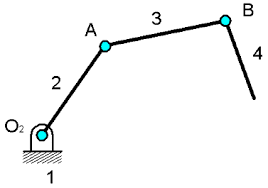
\includegraphics[scale=1]{imag5.png} 
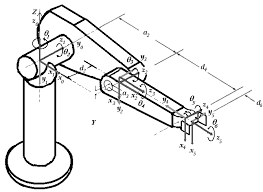
\includegraphics[scale=1]{imag8.png}\\\\\\\\\\\\\\\\\\\\\\\\\\\\\\\\\\\\\\\\\\\\\\

\tableofcontents

\section{Teorema de Euler sobre rotación:}
En geometría hay diferentes formalizaciones para expresar una rotación en tres dimensiones como una transformación matemática. Este concepto se aplica a la mecánica clásica, donde la cinemática rotacional (o angular) es la ciencia que describe cuantitativamente un movimiento puramente rotativo. La orientación de un objeto en un instante dado, ya que se define como una rotación imaginaria a partir de una ubicación de referencia en el espacio, en lugar de una rotación realmente observada de una ubicación anterior en el espacio.\\

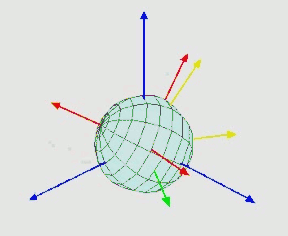
\includegraphics[scale=1]{xyz.PNG} \\
Hemos definido como un movimiento rígido que deja un punto fijo. Euler demostró que esto implica que no hay un solo punto fijo, sino toda una recta que pasa por O. Esta recta es el llamado eje de rotación.\\\\
La demostración se basa en que debe haber un vector no afectado por la rotación, esto es,\\

\includegraphics[scale=1]{Ru.PNG} \\
Si este vector u existe, cualquier múltiplo de él tampoco se verá afectado, con lo que obtenemos toda una recta que pasa por O.\\
En términos algebraicos esto equivale a decir que existe un auto valor unidad, siendo u el auto vector correspondiente. La condición para que ello ocurra es que\\
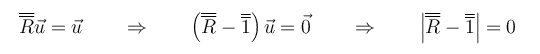
\includegraphics[scale=1]{Ru2.PNG} \\
Veamos que es cierto:\\
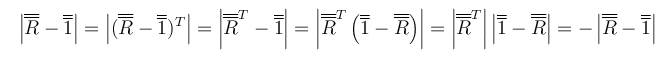
\includegraphics[scale=1]{Ru3.PNG} \\
Y por tanto\\
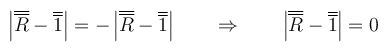
\includegraphics[scale=1]{Ru4.PNG} \\
Por tanto existe el autovalor unidad, y el autovector correspondiente nos da el eje de rotación.

Esto nos da otra forma de parametricar las rotaciones: con dos ángulos (por ejemplo los de las coordenadas esféricas) damos la orientación de este vector director y con un tercer ángulo medimos cuánto ha girado el sólido en torno al eje.\\

Como consecuencia del teorema de Euler, cualquier vector perpendicular al eje de giro sigue siendo perpendicular tras la rotación. Si el vector v2 se transforma en el v.\\\\
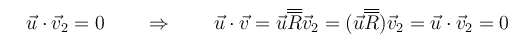
\includegraphics[scale=1]{Ru5.PNG} \\
Cualquier otro vector podrá descomponerse en una parte paralela al eje de giro (que no se verá afectada por la rotación) más una parte ortogonal al eje (que gira un cierto ángulo en torno al eje, manteniéndose ortogonal).\\\\

De acuerdo con el teorema de rotación de Euler, la rotación de un cuerpo rígido (o sistema de coordenadas tridimensional con el origen fijo) se describe mediante una única rotación respecto a un determinado eje. Dicha rotación se puede describir de forma única mediante un mínimo de tres parámetros reales. Sin embargo, por varias razones, hay varias formas de representarlo. Muchas de estas notaciones utilizan más del mínimo necesario de tres parámetros, aunque cada una de ellas tiene solo tres grados de libertad.\\\\
Un ejemplo donde se usa la representación de las rotaciones es en la visión artificial, donde un observador automático necesita rastrear un objetivo. Si se considera un cuerpo rígido, asociado con tres vectores unitarios ortogonales fijados a su cuerpo (que representan los tres ejes del sistema de coordenadas locales del objeto). El problema básico es especificar la orientación de estos tres vectores unitarios, y por lo tanto del cuerpo rígido, con respecto al sistema de coordenadas del observador, considerado como una ubicación de referencia en el espacio.\\\\

\section{Eje y ángulo de Euler (vector de rotación)}
Por el teorema de rotación de Euler, se sabe que cualquier giro se puede expresar como una sola rotación sobre algún eje. El eje es el vector unitario (único si se exceptúa su signo) que permanece sin cambios por efecto de la rotación. La magnitud del ángulo también es única, y su signo está determinado por el signo del eje de rotación.\\\\
El eje se puede representar como un vector unitario tridimensional\\
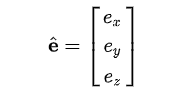
\includegraphics[scale=1]{matriz.PNG} \\

y el ángulo por un escalar 0(theta).\\
Como el eje está normalizado, solo tiene dos grados de libertad. El ángulo agrega el tercer grado de libertad a esta notación de la rotación.\\

Se puede expresar la rotación como un vector de rotación, o vector de Euler, un vector tridimensional no normalizado cuya dirección especifica el eje y cuya longitud es 0,  r= 0é.\\
El vector de rotación es útil en algunos contextos, ya que representa una rotación tridimensional con solo tres valores escalares (sus componentes), que representan los tres grados de libertad. Esto también es cierto para representaciones basadas en secuencias de tres ángulos de Euler (véase más adelante).\\

Si el ángulo de rotación 0 es cero, el eje no está definido de forma única. La combinación de dos rotaciones sucesivas, cada una representada por un eje y un ángulo de Euler, no es sencilla y, de hecho, no satisface la ley de la adición de vectores, lo que muestra que las rotaciones finitas no son realmente vectores. Es mejor emplear la notación de la matriz de rotación o la del cuaternión, calcular el producto y luego volver a convertirlo en el eje y ángulo de Euler.\\
\section{Rotaciones de Euler}
La idea detrás de las rotaciones de Euler es dividir la rotación completa del sistema de coordenadas en tres rotaciones constitutivas más simples, llamadas precesión, nutación y rotación intrínseca, siendo cada una de ellas un incremento en uno de los ángulos de Euler. Obsérvese que la matriz externa representará una rotación alrededor de uno de los ejes del marco de referencia, y la matriz interna representa una rotación alrededor de uno de los ejes del marco en movimiento. \\La matriz central representa una rotación alrededor de un eje intermedio llamado línea de nodos.\\\\

Sin embargo, la definición de los ángulos de Euler no es única y en la bibliografía se utilizan muchas convenciones diferentes. Estas convenciones dependen de los ejes sobre los que se realizan las rotaciones y de su secuencia (ya que las rotaciones no son conmutativas).\\\\

La convención que se usa generalmente se indica especificando los ejes sobre los cuales se realizan las rotaciones consecutivas (antes de ser compuestas), refiriéndose a ellas mediante el índice (1,2,3) o la letra (x,y,z). Las comunidades de ingeniería y robótica suelen utilizar los ángulos de Euler 3-1-3. Obsérvese que después de componer las rotaciones independientes, ya no giran alrededor de su eje. La matriz más externa rota las otras dos, dejando la segunda matriz de rotación sobre la línea de nodos y la tercera en un marco que se mueve con el cuerpo. Hay 3 x 3 x 3 = 27 posibles combinaciones de tres rotaciones básicas, pero solo 3 x 2 x 2 = 12 de ellas se pueden usar para representar rotaciones 3D arbitrarias como ángulos de Euler. Estas 12 combinaciones evitan rotaciones consecutivas alrededor del mismo eje (como XXY), lo que reduciría los grados de libertad que se pueden representar.\\\\

Por lo tanto, los ángulos de Euler nunca se expresan en términos del marco externo, o en términos del marco del cuerpo girado en movimiento conjunto, sino en una mezcla. Se utilizan otras convenciones (por ejemplo, la matriz de rotación o los cuaterniones) para evitar este problema.\\\\\\\\\\\\\\\\\\\\\\\\\\\\\\\\\\\\\\\\\\\\\\\\\\\\\\\\\\\\\\\\\\\\\\\\\\\\\\\\\\\\\\\\\\\\\\\\\\\\\\\\\\\\\\\\\\\

\section{Bibliografía:}

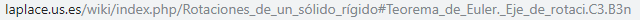
\includegraphics[scale=1]{bib.PNG} 
















\end{document}